\begin{figure}[!t]
	\centering
	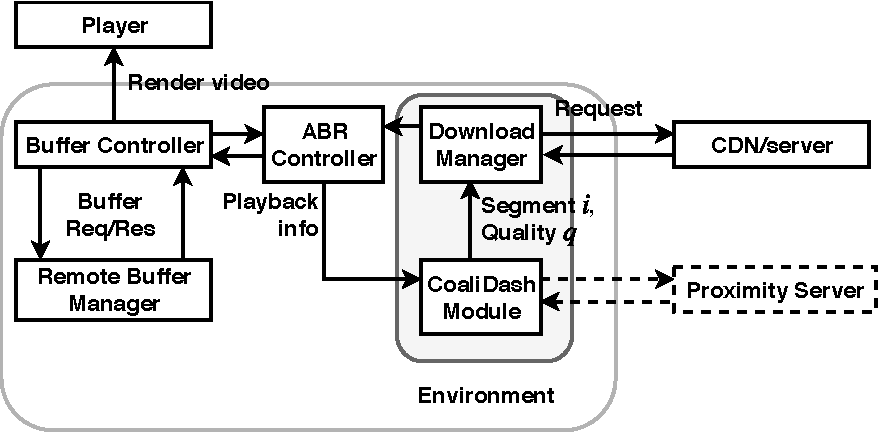
\includegraphics[width=0.8\linewidth]{img/PlayerDiagram}
	\caption{\label{fig:playerdiagram} Architectural Components for Federated Live Streaming over DASH}
\end{figure}

\section{System Model for Federated Live Streaming}
\label{section:systemDesign}
%In our approach, we are trying to exploit the fact that many users watch the same video simultaneously. If we can connect those many users in a controlled peer-to-peer network, then they can share video segment downloaded by a player to another. The traditional way to employ peer-to-peer network in video streaming is to search and fetch method. Here, the player has to search for the location of a content in the network and fetch the content from that particular peer. Although it is working and it can reduce server load to an extent, we like to do it in more methodically.
In a standard DASH based streaming environment, a content server keeps the entire video in multiple quality levels. The video files are divided into many small segments, and every segment is encoded with multiple supported quality levels. Most of the time, the duration of all the segments across different qualities are the same. In case of live streaming, the content server populates segments on the fly as the stream progresses. Depending on the network condition, a DASH-based streaming player downloads segments of the desired quality level and renders them.
In contrast to the client-server architecture followed in DASH, FLSD forms multiple coalitions of players who want to watch a live video in similar quality levels and share an environment with similar average network quality (for example, they are under the same local area network or share a common network gateway), although the network quality of individual players in the coalition can fluctuate over time. Once the coalition is formed, it employs a scheduling policy to download and share the video segments by different players in the coalition at different times. The advantage of this scheme is that a player already knows from whom it is supposed to get the next video content, based on the scheduling algorithm.  
%\notesc{A very brief description (one-two lines) of DASH should come up -- people should understand what is a video segment, and how they are downloaded. Also the perspective of DASH in live streaming should come here. } 


FLSD has three system components as shown in Fig.~\ref{fig:playerdiagram}. (1) {\bf Streaming Server:} The streaming server is a content delivery network (CDN) server which encodes the live videos and hosts the video segments.
%{\bf Tracker:} A tracker is an integral part of the system. It is similar to the tracker used in BitTorrent. However, with few modifications. Here a tracker keeps track of players and associated groups in the system. Whenever a player request for other players, it returns potential neighbours from one or more group to the player. A player does not need to stay connected with the tracker all the time. However, it has to inform every event related to the group, i.e. with which group it got connected, playback quality level and so on.
(2) {\bf Proximity Server:} It keeps information about the players who observe the same video.
It can be noted that any existing video streaming client (or even the streaming server) can work as a proximity server as well. 
(3) {\bf Player:} A player renders the video as well as creates and maintains the coalition. Each player consists of three modules -- i) \textit{Playback}, ii) \textit{Environment}, and iii) \textit{Adaptive Bit Rate} (ABR). 
%Fig.~\ref{fig:playerdiagram} depicts the different components and modules of the FLSD system.
%\notesc{Give a figure explaining the architecture.}
%These modules are independent of each other and can be replaced with a similar module.
% 
A {\it Playback} module keeps track of the playback buffer and the playback time. Each Player has limited buffer capacity; it cannot store the next segment unless it has enough space in the buffer. Every time it receives a segment, the playback module asks the {\it ABR} module for the next quality level and the sleep-time before it can start downloading.
The {\it ABR} module calculates the next quality level and the sleep-time. We can use any existing ABR algorithm for this module. In our implementation, we can choose from Rate Based, Bandwidth-Based, BOLA, MPC and Pensieve adaptation algorithms. The sleep-time indicates at what frequency a player should download the content from the streaming server.  The {\it ABR} module calculate the sleep-time in such way so that the {\it Environment} module, as described next, completes downloading the current segment exactly when the player frees up enough space for the next segment. The {\it Environment} module is responsible for downloading the segments. It predicts the download time based on the network condition and generates the next event based on the download time.
%However, this is not a strict policy. It can ignore the player decision and download segment from anywhere it wants, and any time it wants. Although it can not push a segment to the {\it Player} if the player buffer is full.
%\end{itemize}
The {\it Environment} module forms a coalition with the nearby players and shares segments among other players in the coalition, following a distributed policy enforcement principle. 
%Next we discuss the details of the coalition formation and collaborative streaming mechanism used in FLSD.
%We describe the group formation and group management in section \ref{sec:groupDesign}.
